  \subsection{Valores límites de detección de sintonía}

    Partiendo de la experiencia previa, se determinará los Limites de la frecuencia 
    de sintonía. Para ello, se ajusta el dial del receptor al valor mínimo 
    (\(88[Mhz]\)) y posteriormente se ajusta la perilla de de frecuencia del generador 
    de barrido hasta que se pueda visualizar en el osciloscopio la curva de respuesta 
    del detector. A continuación, se selecciona el rango de frecuencias \textbf{D} 
    del generador de marca y se ajusta la marca para que este en el medio de la 
    curva de respuesta como se ve en la Figura \ref{fig:FrecMintSint}.   
      \begin{figure}[H]
        \centering
        \begin{subfigure}[ht]{0.48\textwidth}
          \frame{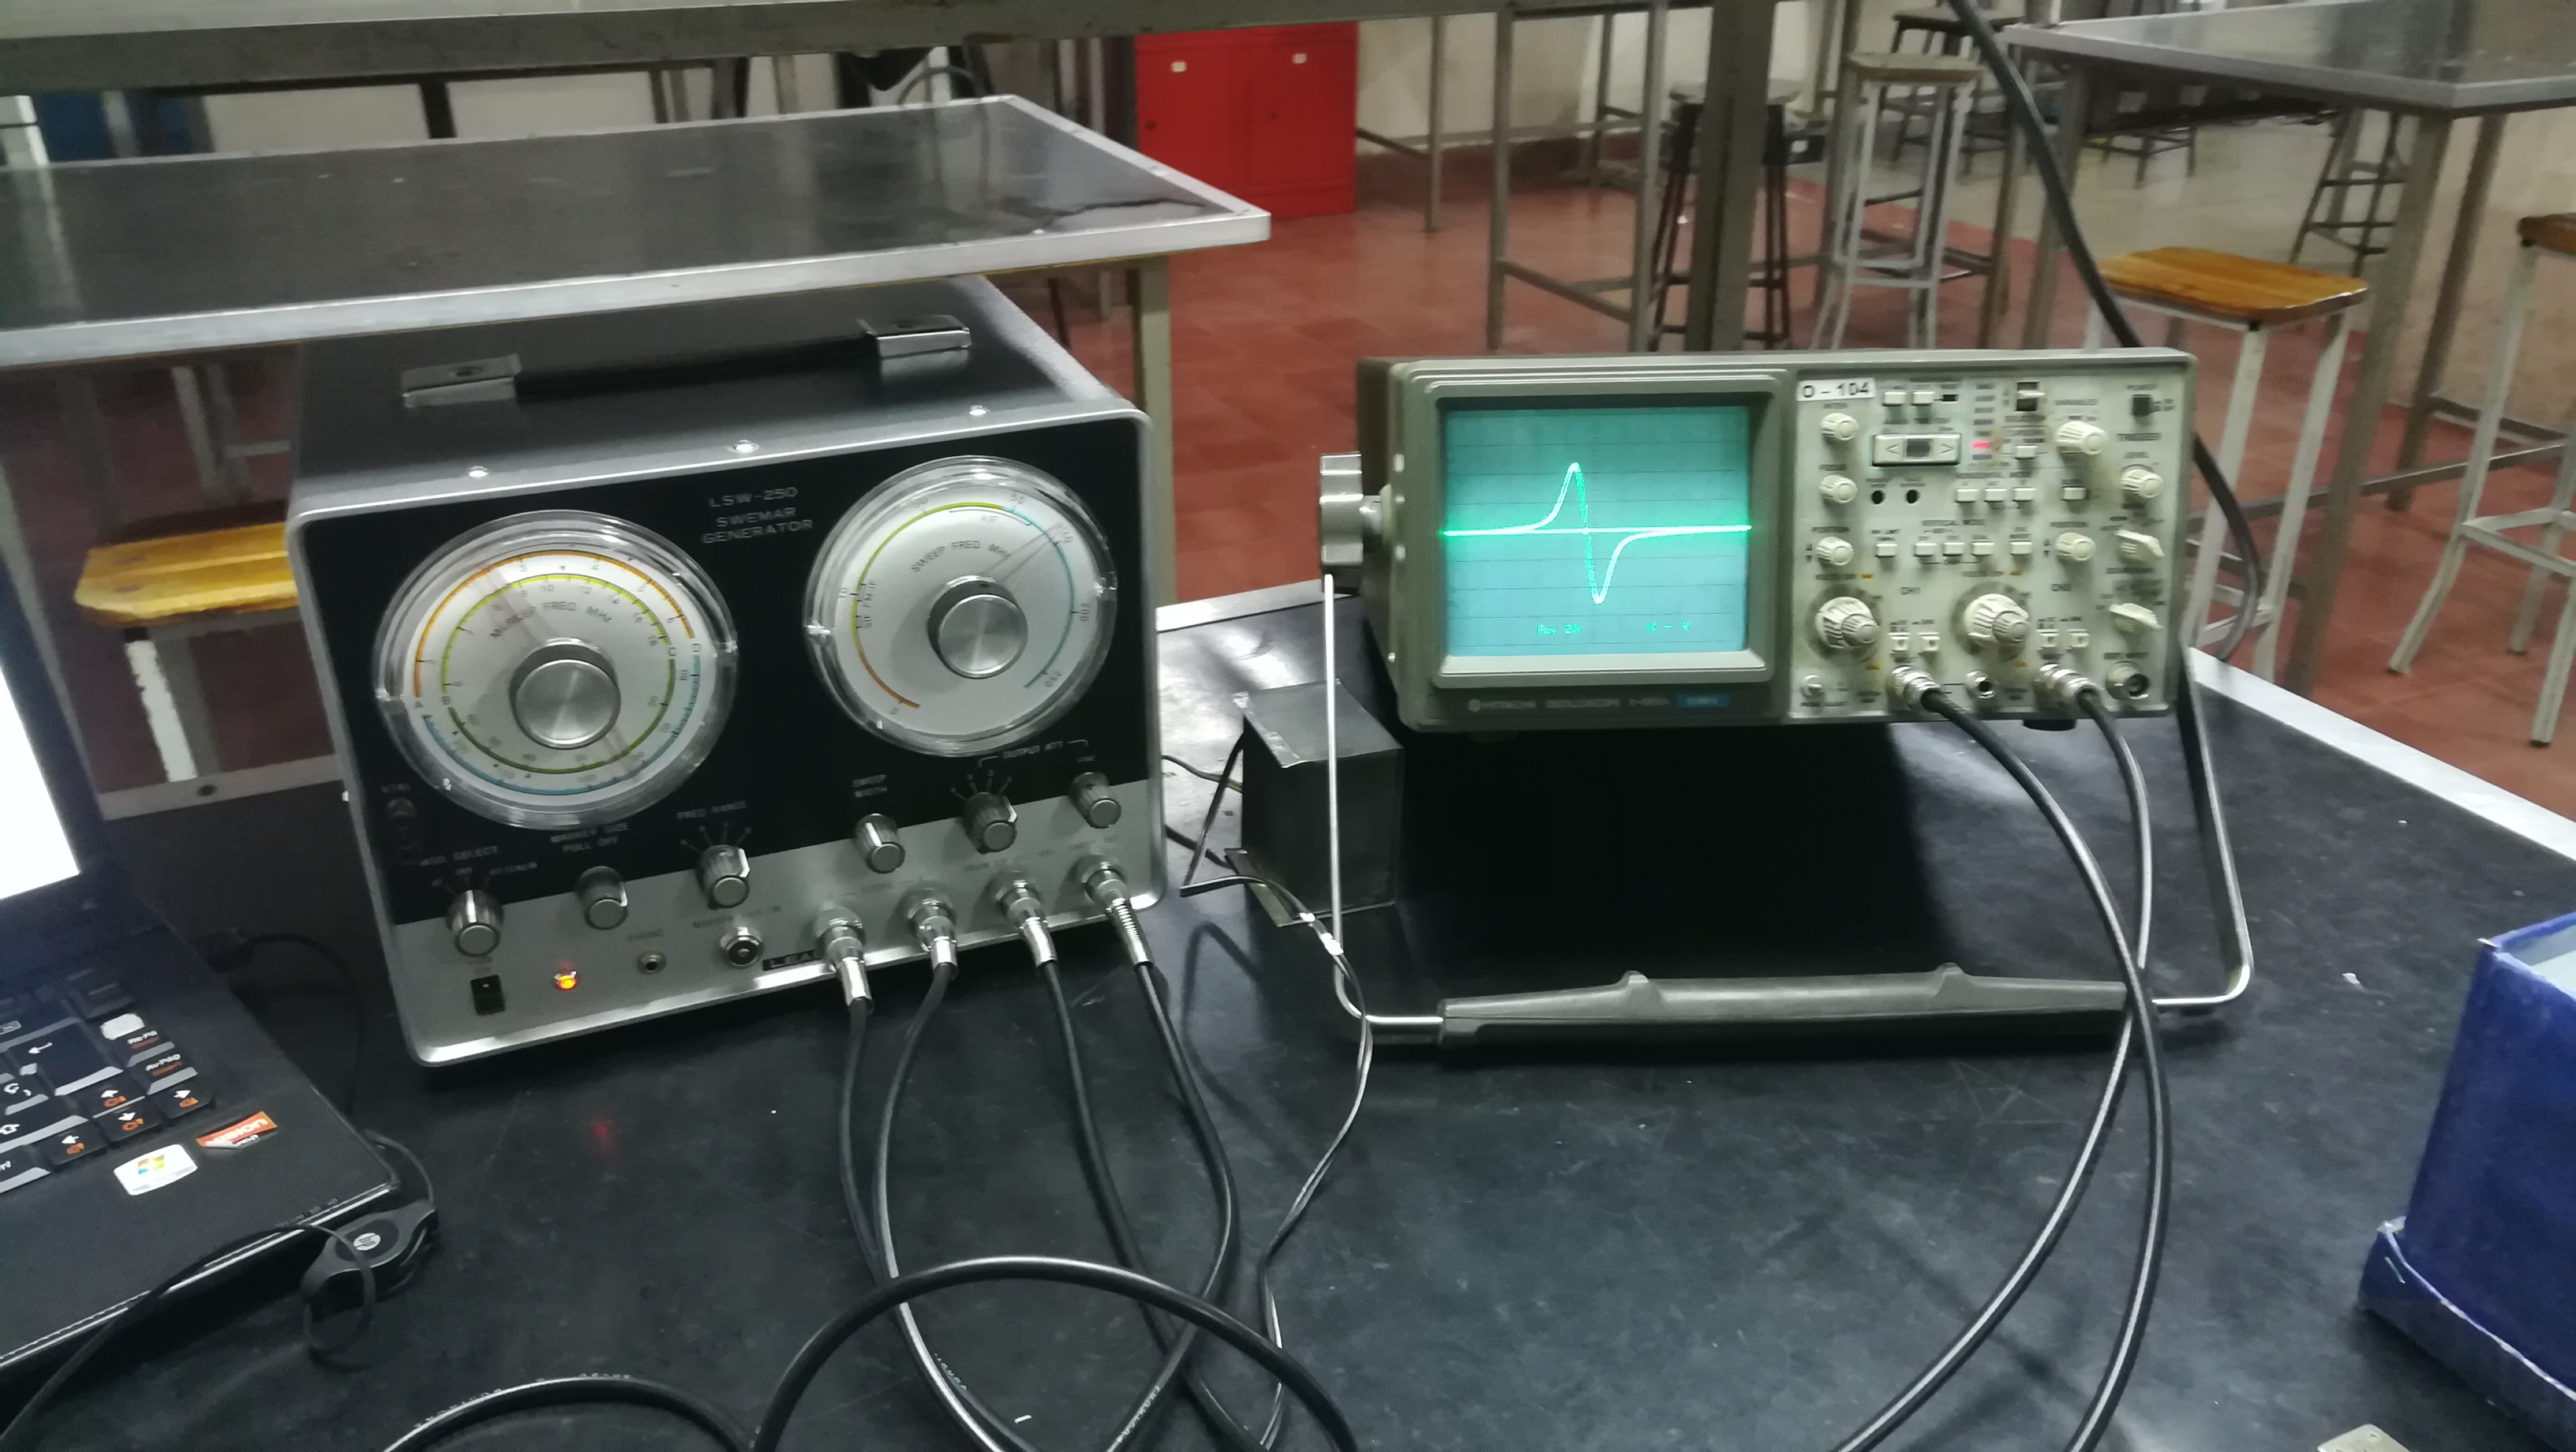
\includegraphics[width=\textwidth]{Imagenes/ActividadPractica/LimitesDeDetecDeSintonia/Exp3.8_FsintoniaMIN_InstrumentosConMarcaAlMedio.jpg}}
          \caption{Medición de frec. mínima de sintonía.}
          \label{fig:FrecMinSintConGen}
        \end{subfigure}
        \hfill 
        \begin{subfigure}[ht]{0.48\textwidth}
          \frame{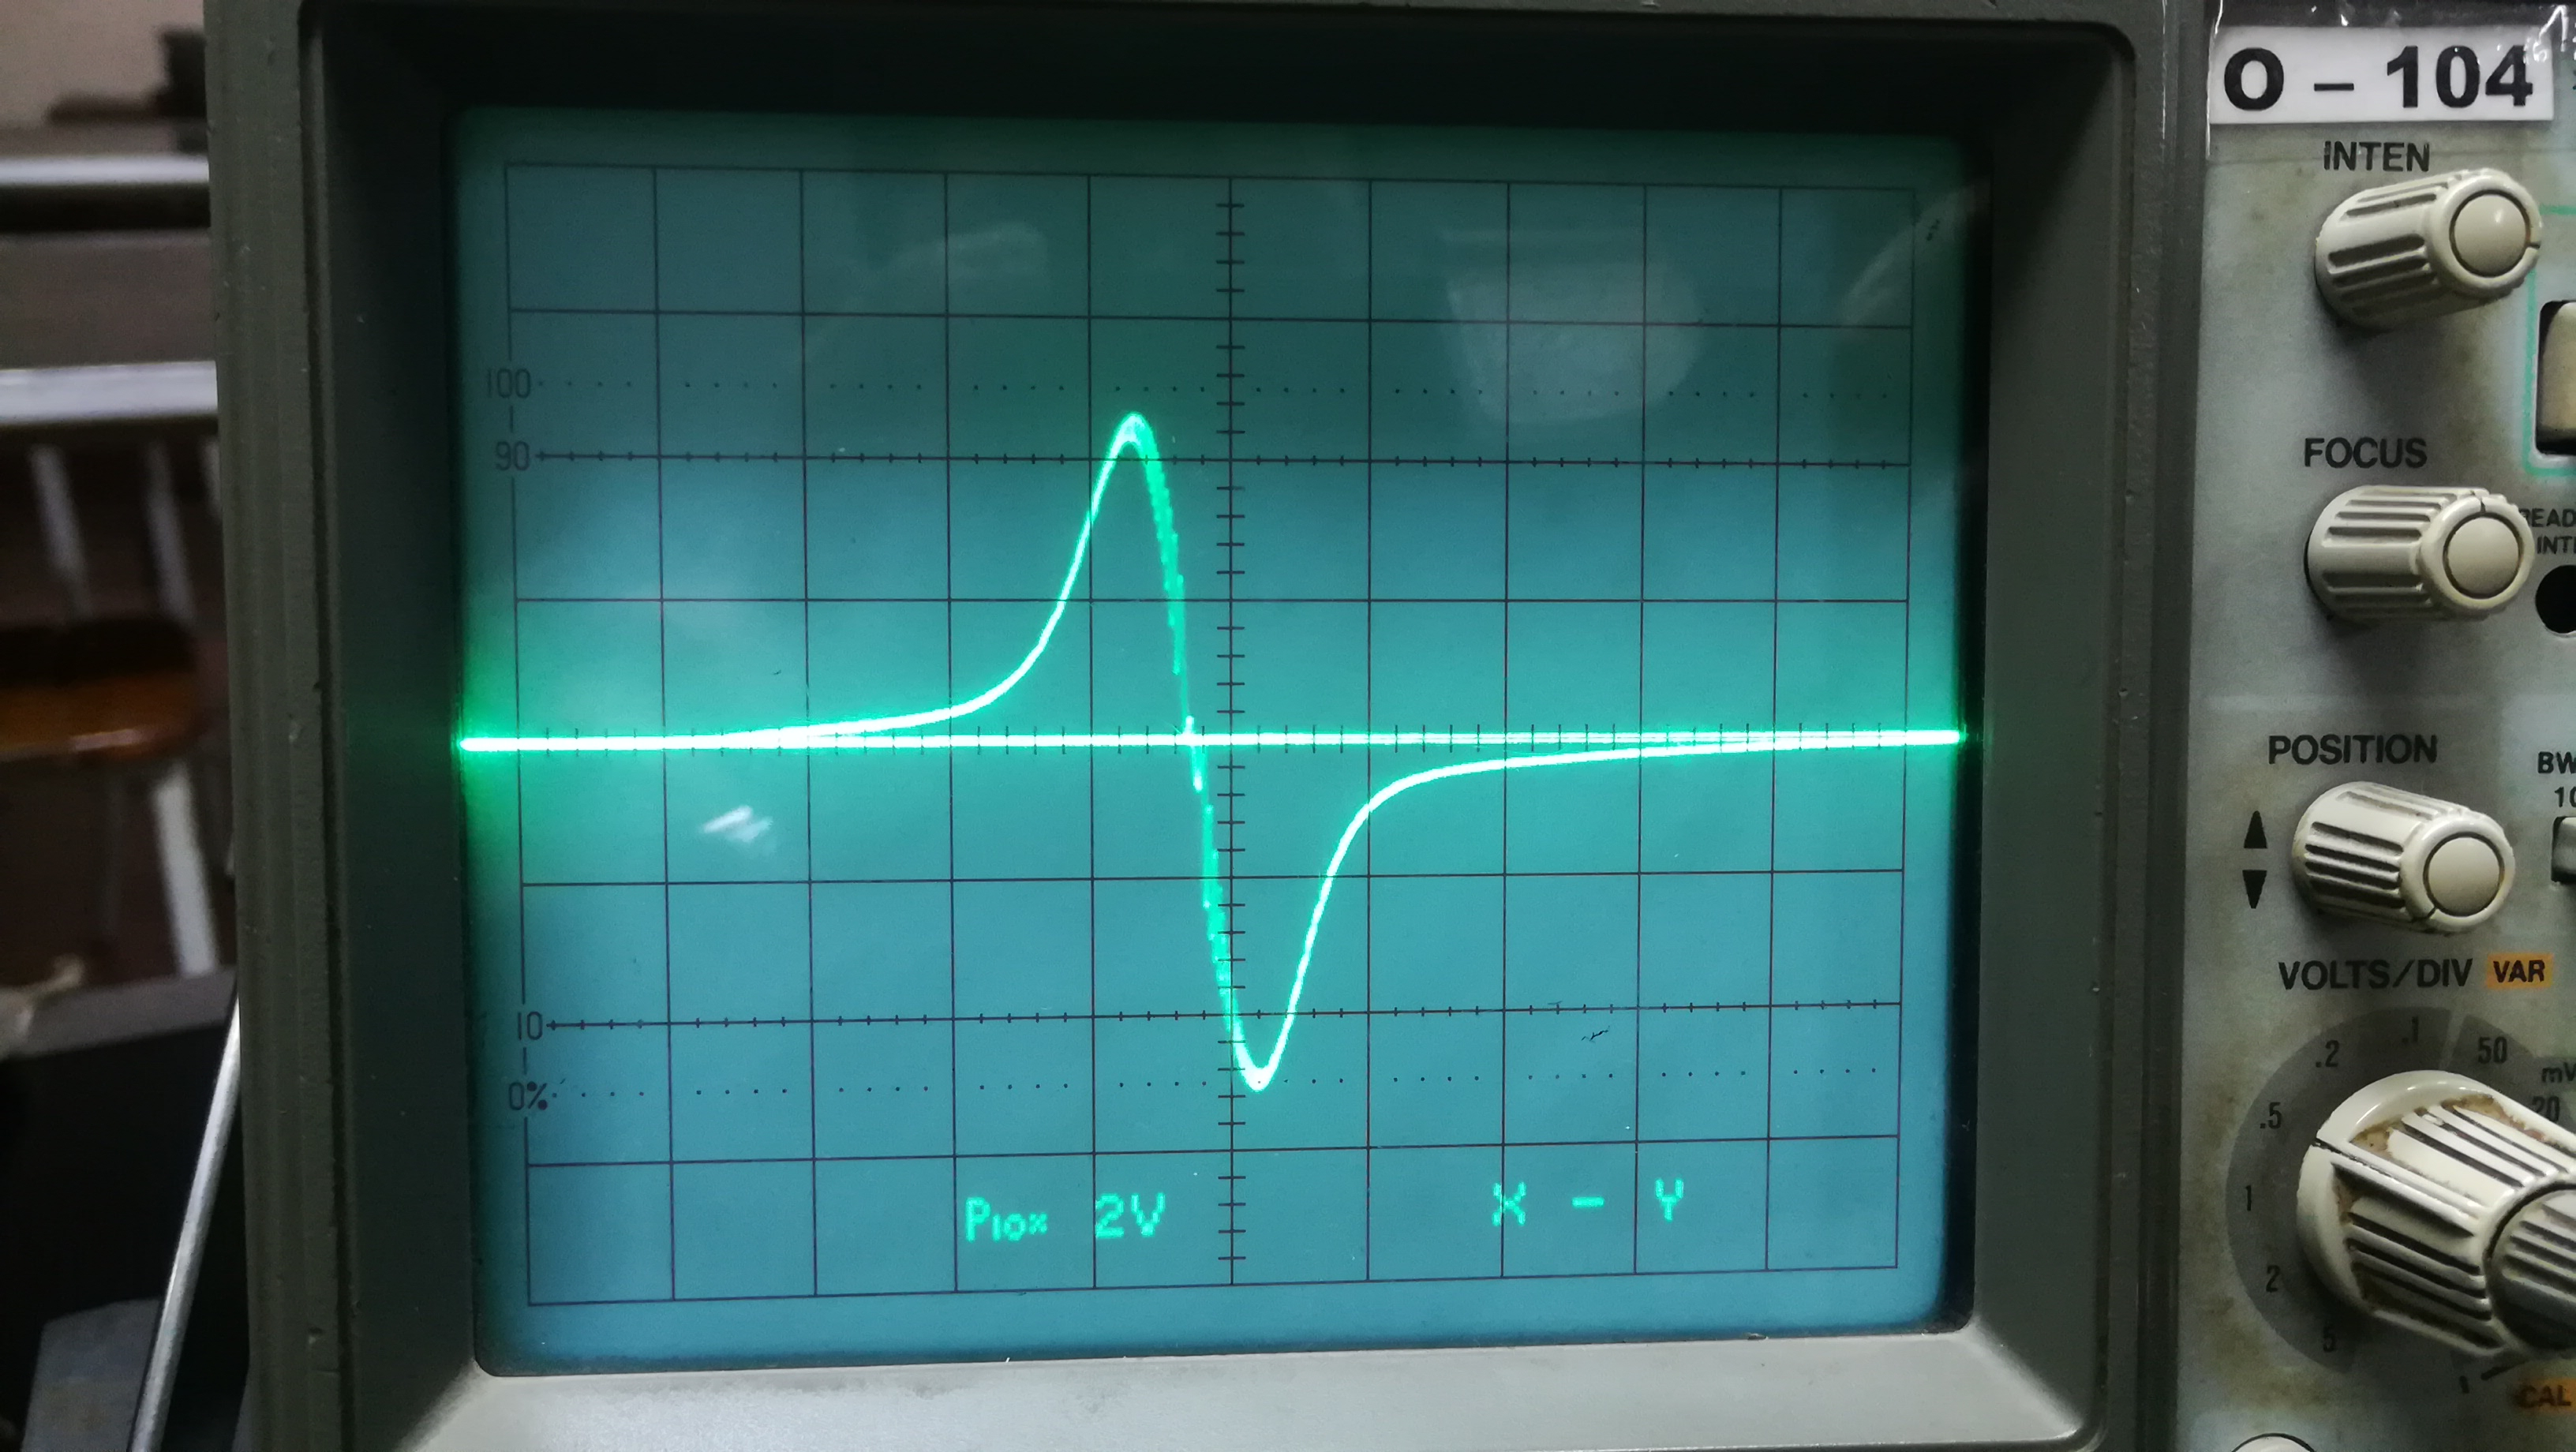
\includegraphics[width=\textwidth]{Imagenes/ActividadPractica/LimitesDeDetecDeSintonia/Exp3.9_FsintoniaMIN_MarcaEnElMedio.jpg}}
          \caption{Valor de  \(Frec_{min_{sint}} = 85~[Mhz]\).}
          \label{fig:FrecMinSintValor}
        \end{subfigure}
        \caption{Detección de frecuencia mínima de sintonía.}
        \label{fig:FrecMintSint}
      \end{figure}

    Ahora, el dial del receptor se lo lleva al valor máximo (\(108~[Mhz]\)) y se 
    repite los mismos pasos previamente realizados. De esta manera se determina el valor 
    del límite máximo para la frecuencia de sintonía como se observa en la Figura 
    \ref{fig:FrecMaxtSint}.  
      \begin{figure}[H]
        \centering
        \begin{subfigure}[ht]{0.48\textwidth}
          \frame{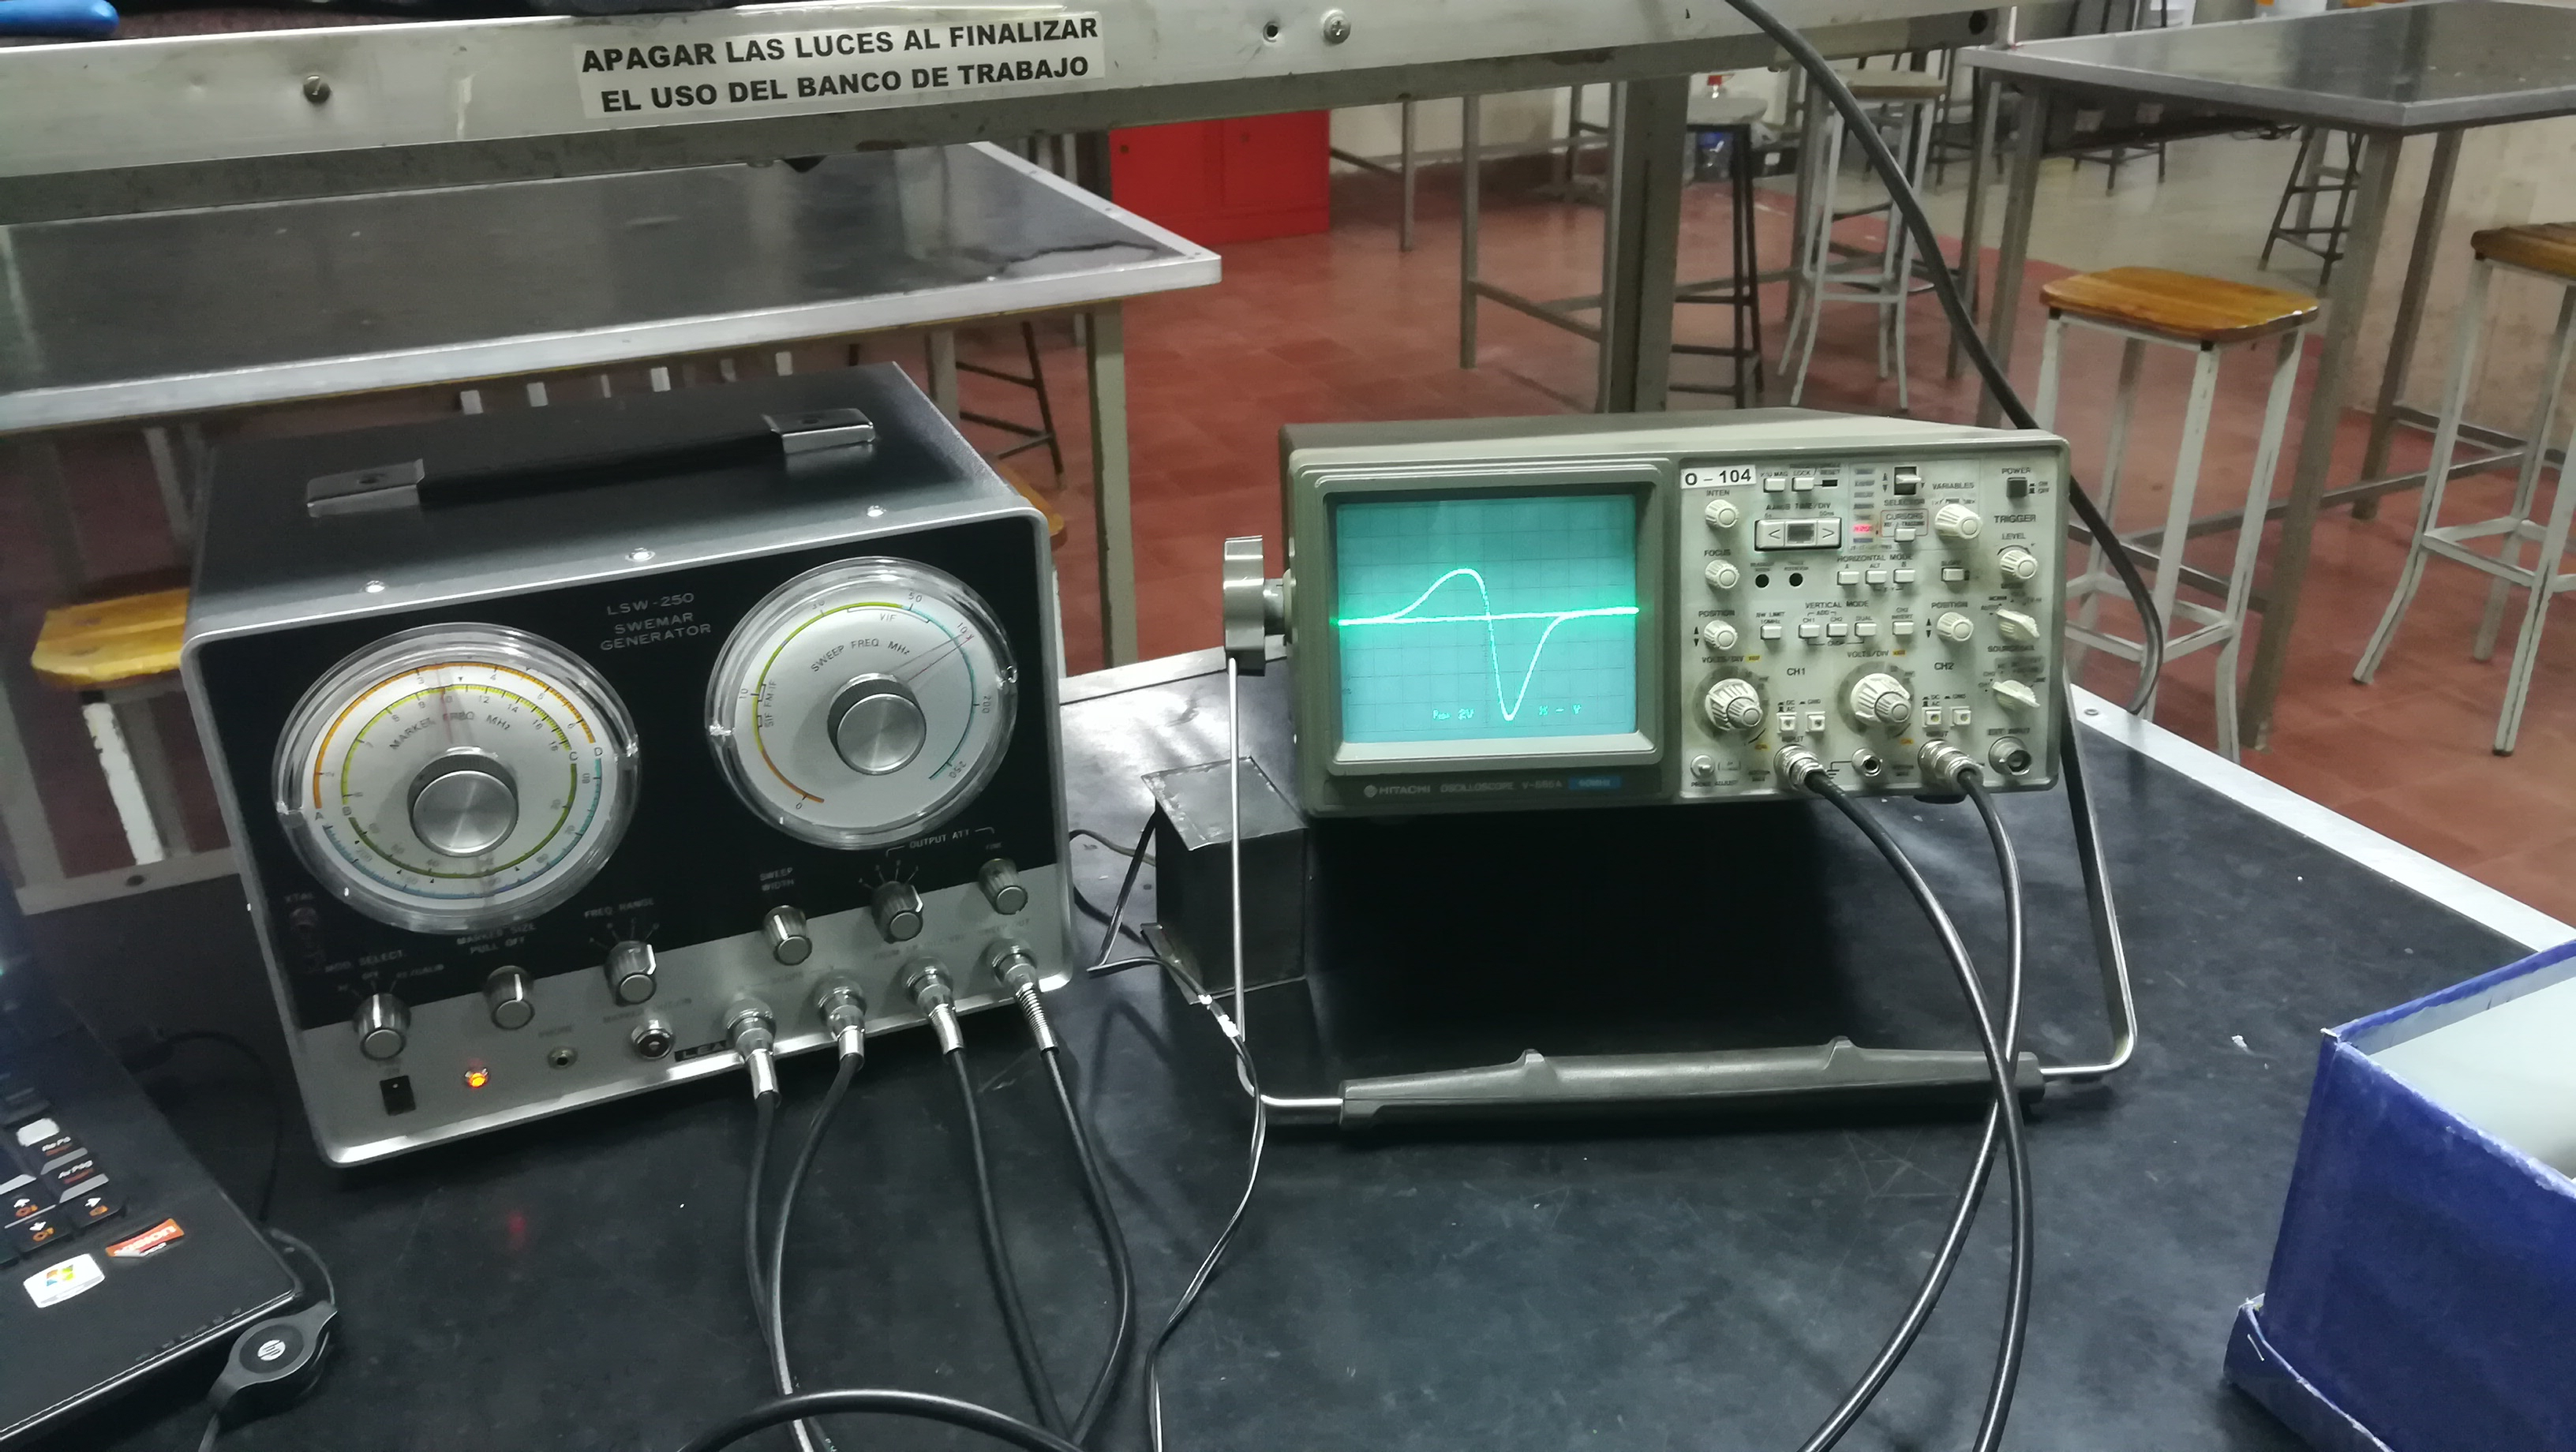
\includegraphics[width=\textwidth]{Imagenes/ActividadPractica/LimitesDeDetecDeSintonia/Exp3.3_FsintoniaMAX_InstrumentosConMarcaAlMedio.jpg}}
          \caption{Medición de frec. máxima de sintonía.}
          \label{fig:FrecMaxSintConGen}
        \end{subfigure}
        \hfill 
        \begin{subfigure}[ht]{0.48\textwidth}
          \frame{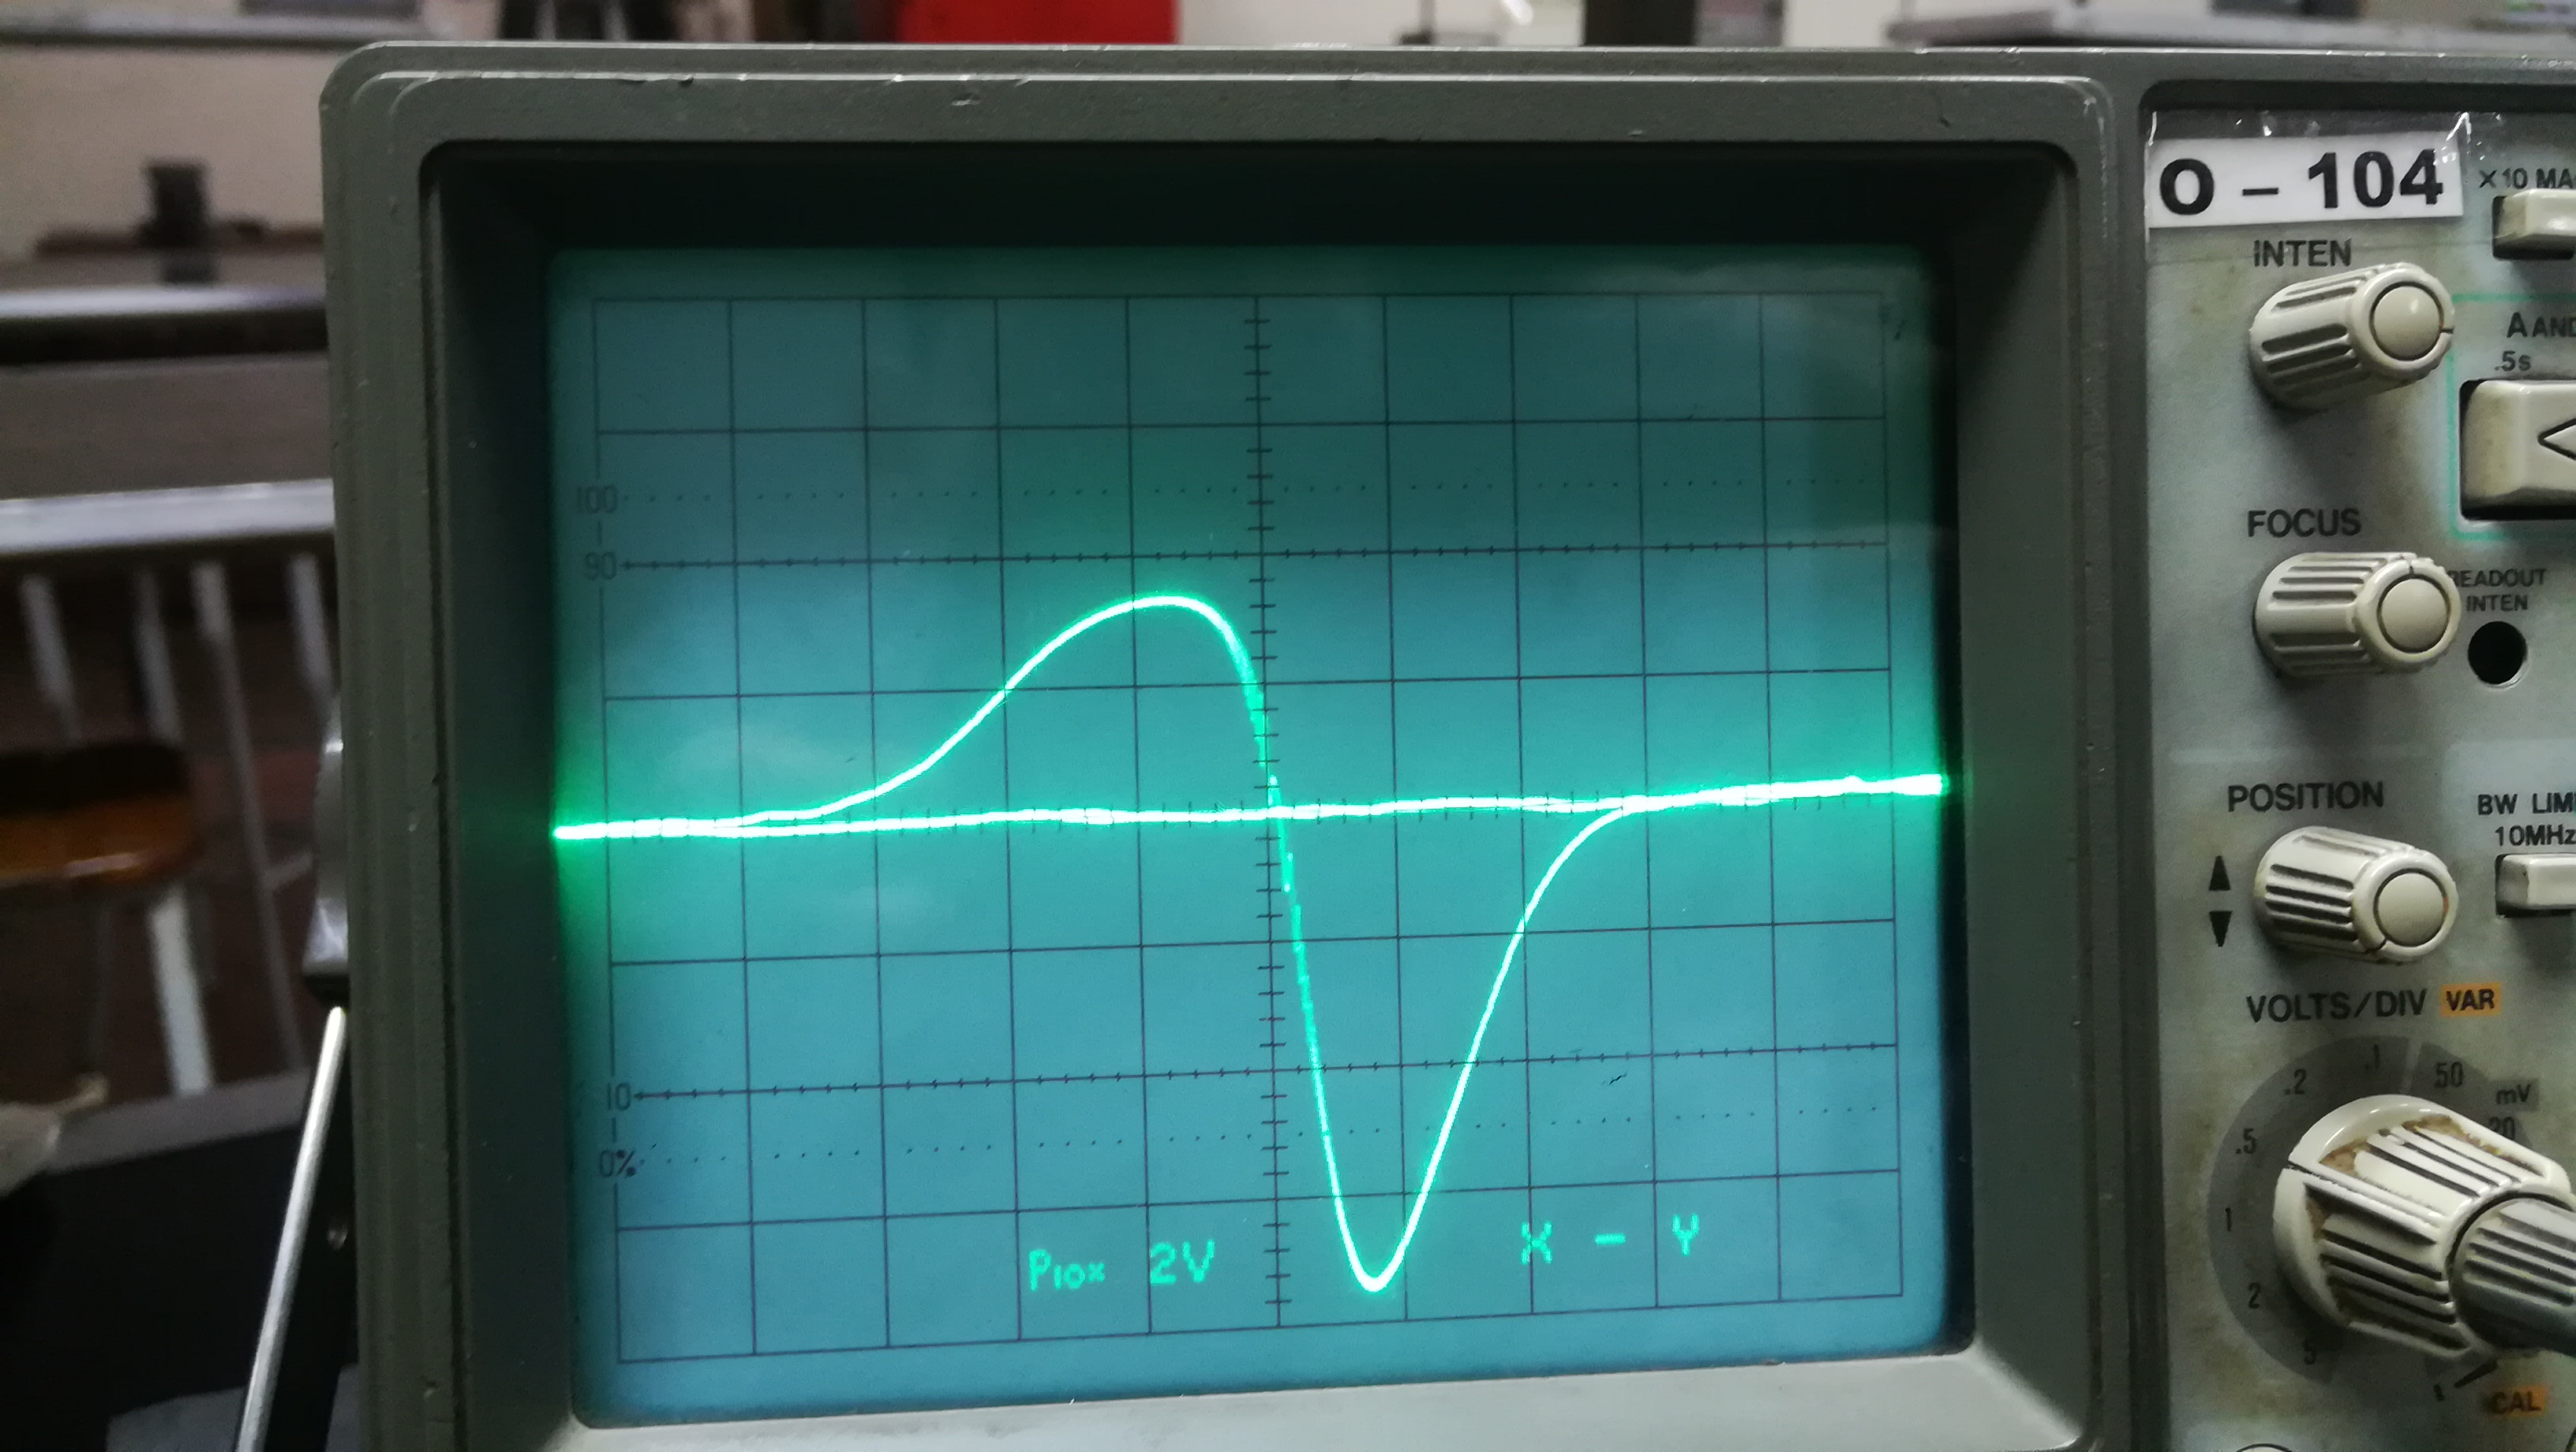
\includegraphics[width=\textwidth]{Imagenes/ActividadPractica/LimitesDeDetecDeSintonia/Exp3.4_FsintoniaMAX_MarcaEnElMedio.jpg}}
          \caption{Valor de  \(Frec_{max_{sint}} = 104~[Mhz]\).}
          \label{fig:FrecMaxSintValor}
        \end{subfigure}
        \caption{Detección de frecuencia mínima de sintonía.}
        \label{fig:FrecMaxtSint}
      \end{figure}

      Por último se tabula los valores obtenidos en la Tabla \ref{tab:MedFrecSinto}.

        \begin{table}[H]
          \small
          \centering
          \begin{tabular}{c c}
              \toprule
              \textbf{Frec. sintonía mínima} &  \textbf{Frec. sintonía máxima} \\ 
              \midrule
              \(85~[Mhz]\)   &   \(104~[Mhz]\) \\ 
              \bottomrule
          \end{tabular}
          \caption{Mediciones de limites de frec. de sintonía.}
          \label{tab:MedFrecSinto}
        \end{table}

        